\documentclass[acmsmall]{acmart}

% Packages
\usepackage{booktabs} % For formal tables
\usepackage{enumitem}
\usepackage{pgfplots}
\usepackage[ruled]{algorithm2e} % For algorithms
\renewcommand{\algorithmcfname}{ALGORITHM}

% Format
\SetAlFnt{\small}
\SetAlCapFnt{\small}
\SetAlCapNameFnt{\small}
\SetAlCapHSkip{0pt}
\IncMargin{-\parindent}

% Metadata Information
\acmJournal{N.A.}
\acmVolume{N.A.}
\acmNumber{N.A.}
\acmArticle{1 N.A. }
\acmYear{2017}
\acmMonth{4}

\acmBadgeR[http://ctuning.org/ae/ppopp2016.html]{ae-logo}

% Copyright
\setcopyright{rightsretained}

% DOI
\acmDOI{0000001.0000001}

% Document starts
\begin{document}
\title{A Brief Survey on Event Detection Methods for Geo-social Media Data}
\author{Richard Wen}
\orcid{0000-0002-8904-8152}
\affiliation{%
  \institution{Ryerson University}
  \streetaddress{350 Victoria Street}
  \city{Toronto}
  \state{ON}
  \postcode{M5B2K3}
  \country{CA}}

\begin{abstract}
In this survey, 5 research papers from 2013 to 2017 were selected from the ACM digital library by using automated and manual criteria. These 5 papers were summarized to present commonly used raw data structures and processed data structures for geo-social media event detection. It was found that frequency-based event detection methods in the selected papers were commonly implemented with statistical measures to determine irregular frequencies in geo-social media data. These irregular location referenced frequencies were determined as events. In order for event detection methods to take advantage of geo-social media data, algorithms must ideally be efficient, scalable, and adaptable. For future work, incorporating video and sound data, integrating web-based knowledge resources, standardizing data structures, and working towards event prediction were suggested to improve and advance event detection methods for geo-social media data.
\end{abstract}

\keywords{survey, review, geo, location, social, media, event, detection}

\thanks{
This work fulfills the requirements of the Knowledge Discovery course instructed by Dr. Cherie Ding during Winter 2017 at Ryerson University. This work used the ACM paper template for journals, but was not intended to be submitted as a publication to the ACM digital library. \textbf{References (such as journal name, article name, volume number, and issue number) to this work are used for template purposes and should not be cited as a publication}.
}


\maketitle

% ============
% Introduction
% ============
\section{Introduction} \label{introduction}

The wide usage of social media platforms, such as Twitter \cite{Twitter:2017} and Facebook \cite{Facebook:2017}, on mobile devices have enabled millions of people to exchange text, images, sound recordings, and videos from any location with wireless internet connection. The Global Positioning System (GPS) in mobile devices further enhances these data with coordinate references that provide information on the location of social media users. Massive amounts of social media data with locational references, referred to as geo-social media data, are then made possible with the integration of GPSes and mobile devices. The massive volumes of geo-social media data are created in real-time from millions of users everyday. This data is capable of providing information on real-world events such as traffic jams, festivals, disasters, and news in near real-time from around the world. Events can be known or predicted before news reports are released for situations in which time-sensitive information is important such as natural disasters or terrorist attacks. However, the data is subject to human errors, noise, changes, and lack of well-defined structures. This survey seeks to provide a review of research papers in which the objective is to create generalized methods for handling data and detecting real-world events from geo-social media sources.

  The goal of this survey is to provide a review that summarizes and synthesizes recent event detection methods for geo-social media data. The review is done by using both automated and manual criteria to filter research papers from the Association for Computing Machinery (ACM) digital library. These filtered papers are then selected to be summarized and compared for structures of data, methods, applications, and examples that apply to event detection for geo-social media data. Finally, a discussion of challenges, proposed improvements, and future directions is provided to address the implications of the papers.

  The remaining sections are then organized as follows:

\begin{itemize}
  \item Section \ref{methods} details the methods used for paper selection and summarizing selected papers
  \item Section \ref{results} presents the results of the paper selection and summary of the selected papers
  \item Section \ref{discussion} discusses the challenges, proposed improvements, and future directions relative to the selected papers
  \item Section \ref{conclusion} provides concluding remarks and implications
\end{itemize}

% =======
% Methods
% =======
\section{Methods} \label{methods}

This section explains the paper selection requirements and process. A combination of automated and manual criteria was used to discover detailed, relevant, and recent papers for geo-social event detection from an online digital library.

\subsection{Search Criteria} \label{search-criteria}

This survey was based on a selection of papers from the ACM repository. An automated online search query was used to filter for relevant papers in the ACM digital library. An \textit{advanced search} query was used to filter for published papers matching the following criteria:

\begin{enumerate}[label=(\alph*)]
  \item \textbf{Publication}: Published in an ACM proceeding
  \item \textbf{Year}: Published from 2013 to April 17, 2017
  \item \textbf{Keywords}: Contains the following words in any common field: \textit{geo}, \textit{location}, \textit{social}, \textit{media}, \textit{event}
\end{enumerate}

\subsection{Non-search Criteria} \label{non-search-criteria}

Manual "hand-picked" criteria, referred to as the non-search criteria in this survey, were also used to filter for papers after applying the initial search criteria in Section \ref{search-criteria}. The \textit{year} search criteria, criteria (b), was determined by querying backwards in decrements of a year from the April 17, 2017 until a total of 5 relevant papers with more than 7 pages (indicating full papers) were found. The relevancy and paper length requirement from this process was known as the non-search criteria. Relevant papers were required to have research objectives that sought to identify or predict meaningful events with geo-social media data. Relevant papers were also required to provide methods that were generalizable such that the techniques used were not limited to one application field. For example, the relevant papers were required to be applicable to multiple application fields such as healthcare, journalism, and disaster monitoring. The non-search criteria ensured that the selected papers were \textit{detailed} (a), \textit{recent} (b), and \textit{relevant} (c) to the focus of this survey as defined in the following:

\begin{enumerate}[label=(\alph*)]
  \item \textbf{Detailed}: Paper contained detailed explanation of methods and results with the assumption that full papers (papers with more than 7 pages) had this characteristic
  \item \textbf{Recent}: Paper was published within the past 10 years
  \item \textbf{Relevant}: Paper had research objectives in which the goal was to detect or predict events using geo-social media data using generalizable methods
\end{enumerate}

\subsection{Survey Procedure} \label{survey-procedure}

A loosely-defined survey procedure was applied to review the selected papers filtered from the search criteria (Section \ref{search-criteria}) followed by the non-search criteria (Section \ref{non-search-criteria}). The survey procedure involved further reviewing the selected papers by:

\begin{enumerate}[label=(\arabic*)]
  \item \textbf{Identifying} the methods used for detecting or predicting meaningful events
  \item \textbf{Identifying} the data structures appropriate for the methods in (1)
  \item \textbf{Identifying} the example applications or conducted experiments
  \item \textbf{Grouping} similar methods in (1), data structures in (2), and applications or experiments in (3) into summary sections
  \item \textbf{Comparing} the methods, data structures, applications, or experiments contained in each of the summary sections in (4)
  \item \textbf{Discussing} challenges, proposed improvements, and future directions relative to the summary sections in (4) after the comparisons in (5)
\end{enumerate}

% =======
% Results
% =======
\section{Results} \label{results}

This section provides details on the paper selection results and survey procedure as described in Section \ref{methods}. Papers from the years 2013 to 2016 were selected to be reviewed for geo-social event detection methods.

\subsection{Selected Papers} \label{selected-papers}

\begin{figure}
\begin{center}
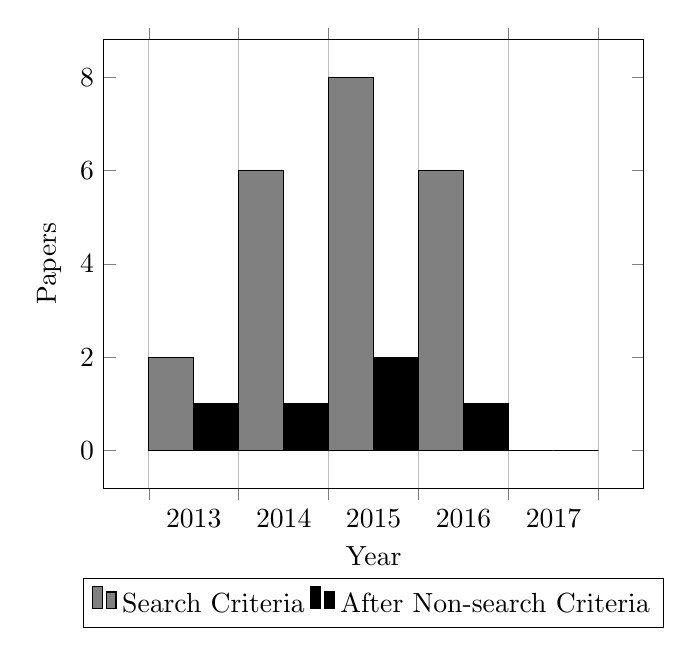
\begin{tikzpicture}
\begin{axis}[
    ylabel=Papers,
    xlabel=Year,
    ybar interval=1,
	xticklabel style={/pgf/number format/1000 sep=,},
	legend style={
	  at={(0.5,-0.20)},
	  anchor=north,
	  legend columns=-1
	}
  ]
  \addplot[color=black, fill=gray] coordinates {(2013,2) (2014,6) (2015,8) (2016,6) (2017,0) (2018,0)};
  \addplot[color=black, fill=black] coordinates {(2013,1) (2014,1) (2015,2) (2016,1) (2017,0) (2018, 0)};
  \legend{\strut Search Criteria, \strut After Non-search Criteria}
\end{axis}
\end{tikzpicture}
\caption{ACM Published Proceeding Papers Found from 2013 to April 17, 2017.}
\label{fig:papersfound}
\end{center}
\end{figure}

The papers after applying the search criteria described in Section \ref{search-criteria} returned 2, 6, 8, 6 and 0 papers for the years 2013, 2014, 2015, 2016, and 2017 respectively. A total of 22 papers from the search criteria were then manually filtered further using the non-search criteria described in Section \ref{non-search-criteria}. A summary of the papers used in this survey by year is shown in (Figure \ref{fig:papersfound}). The papers filtered from the non-search criteria, after initially applying the search criteria, were used in this survey. These 5 papers (ordered by year and then ordered alphabetically) were authored by:

\begin{enumerate}[label=(\arabic*)]
  \item Shirai, Masaharu, and Hiro (2013) \cite{Shirai:2013}
  \item Abdelhaq and Gertz (2014) \cite{Abdelhaq:2014}
  \item Wang and Kankanhalli (2015) \cite{Wang:2015}
  \item Wu et al. (2015) \cite{Wu:2015}
  \item Schubert, Weiler, and Kriegel (2016) \cite{Schubert:2016}
\end{enumerate}

\subsection{Summary of Selected Papers} \label{summary-of-selected-papers}

A summary of the selected papers in Section \ref{selected-papers} was done to provide an overview of event detection methods for geo-social media data. This section provides a briefing of the various data structures, data processing transformations, event detection methods, and applications of geo-social event detection from the selected papers. Each paper used different processed data, but most papers used raw textual data from Twitter, and frequency-based event detection methods.

\subsubsection{Data Structures} \label{data-structures}

\begin{table}
\centering
\caption{Geo-social Media Data Structures for Selected Papers.}
\label{table:structures}
\begin{tabular}{lllll}
\hline
\textbf{Structure} & \textbf{Example} & \textbf{Metadata} & \textbf{Source} & \textbf{Papers} \\ \hline
Textual & \textit{"Some characters"} & \textit{\begin{tabular}[c]{@{}l@{}}time-stamp=2017-04-17 00:00:00\\ coordinates=00.00,00.00\end{tabular}} & Tweets & 5 \\ \hline
Image & \textit{\begin{tabular}[c]{@{}l@{}}0 255 1 25\\ 0 105 1 15\\ 0 33 1 25\end{tabular}} & \textit{\begin{tabular}[c]{@{}l@{}}timestamp=2017-04-17 00:00:00\\ coordinates=00.00,00.00\end{tabular}} & User photos & 2 \\ \hline
\end{tabular}
\end{table}

Geo-social media data were obtained in several different data structures. All 5 of the selected papers utilized textual data with locational reference such as sentences and keywords from social media posts for data filtering and model interpretation. The textual data in the selected papers were obtained as tweets, user posts containing 140 character texts, from Twitter \cite{Twitter:2017} with time-stamps and locational references. For example, the textual data may contain characters \textit{"some character text from a user post"} with metadata containing a time-stamp \textit{"2017-04-17 00:00:00"} (year-month-day hours:minutes:seconds), and coordinates \textit{"0.00, 0.00"} (longitude, latitude) relative to the time and location in which this textual data point was created. Image data from user photos were also used by Shirai et al (2013) \cite{Shirai:2013} and Wang and Kankanhalli \cite{Wang:2015}. This image data contains pixel intensities arranged in a grid-like structure with time-stamps and coordinates metadata representing time and location references. Wang and Kankanhalli \cite{Wang:2015} also integrated external sources of data such as security camera feeds containing videos with locational reference with tweets to enhance the interpretation of model results. Table \ref{table:structures} provides a summary of the data structures used in the selected papers.

\subsubsection{Data Processing} \label{data-processing}

\begin{table}
\centering
\caption{Processed Geo-social Media Data Structures for Selected Papers.}
\label{table:processed}
\begin{tabular}{lllll}
\hline
\textbf{Processed} & \textbf{Example} & \textbf{Metadata} & \textbf{Source} & \textbf{Papers} \\ \hline
Tokens & \textit{"keyword \#tag"} & \textit{timestamp=2017-04-17 00:00} & Tweets & 2 \\ \hline
Geo-tokens & \textit{"!geo0!0!0"} & \textit{timestamp=2017-04-17 00:00} & Tweets & 1 \\ \hline
PST & \textit{\begin{tabular}[c]{@{}l@{}}temp=2017-04-17 00:00\\ loc=00.00,00.00\\ label=human,parade\\ prob=0.8\end{tabular}} & \textit{pointer=id} & \begin{tabular}[c]{@{}l@{}}Tweets\\ User photos\end{tabular} & 1 \\ \hline
Points & \begin{tabular}[c]{@{}l@{}}(00.00,00.00)\\ (01.00,01.00)\end{tabular} & \textit{\begin{tabular}[c]{@{}l@{}}timestamp=2017-04-17 00:00\\ timestamp=2017-04-17 00:01\end{tabular}} & Tweets & 1
\end{tabular}
\end{table}

Various data processing methods were used in the selected papers to handle the loosely defined structures of geo-social media data. Schubert et al. (2016) \cite{Schubert:2016} used grid-based tokenization where important words, known as tokens, were extracted, and coordinates were formatted as tokens, known as geo-tokens, using coordinate grids spaced at every even latitudinal and longitudinal degrees for a study area. For example, a token for \textit{"processing"} is \textit{"process"}, and a geo-token for the coordinates \textit{"0.00, 0.00"} is \textit{"!geo0!0!0"} \footnote{The number after \textit{"!geo"} refers to the index of the coordinate grids.}. The coordinate grids are further expanded to include administrative boundaries such as city or neighborhood boundaries. Wang and Kankanhalli \cite{Wang:2015} used four elements of camera location, temporal information, textual label, and probability that the text labels belong to a topic \footnote{A topic is an abstract representation from textual data. For example, the textual data \textit{"Heading to the concert"} may contain a topic named \textit{"concert"} as a more abstract representation of the text.} to form a uniform data structure called Probabilistic Spatio-temporal (PST) data. PST data also involved word tokenization. Wu et al. (2015) \cite{Wu:2015} used a set of coordinate points with textual data to represent mobility of social media users. For example, a set of coordinate points can be \textit{"(00.00, 00.00) (01.00, 01.00) (02.00, 02.00)"} with each point encased in brackets. The data processing methods sought to unify the raw data structures from Twitter tweets in order to improve consistency and interpretation.  Table \ref{table:processed} provides a summary of the processed data structures used in the selected papers.

\subsubsection{Event Detection} \label{event-detection}

\begin{table}
\centering
\caption{Geo-social Event Detection Methods for Selected Papers.}
\label{table:methods}
\begin{tabular}{llll}
\hline
\textbf{Method} & \textbf{Purpose} & \textbf{Data} & \textbf{Paper} \\ \hline
\begin{tabular}[c]{@{}l@{}}Normalized\\ EWMA\end{tabular} & \begin{tabular}[c]{@{}l@{}}Event detection\\ Real-time\end{tabular} & \begin{tabular}[c]{@{}l@{}}Tokens\\ Geo-tokens\end{tabular} & Schubert et al. (2016) \\ \hline
\begin{tabular}[c]{@{}l@{}}KDE\\ Rel. Score\end{tabular} & \begin{tabular}[c]{@{}l@{}}Event detection\\ Text annotation\end{tabular} & Points & Wu et al. (2015) \\ \hline
\begin{tabular}[c]{@{}l@{}}Entropy\\ Sliding Window\end{tabular} & \begin{tabular}[c]{@{}l@{}}Event detection\\ Word locality\end{tabular} & Textual & Abdelhaq and Gertz (2014) \\ \hline
\begin{tabular}[c]{@{}l@{}}Common Stats\\ Freq. Weights\end{tabular} & \begin{tabular}[c]{@{}l@{}}Event detection\\ Data integration\end{tabular} & \begin{tabular}[c]{@{}l@{}}PST\\ Tokens\end{tabular} & Wang and Kankanhalli (2015) \\ \hline
Camera Orient. & \begin{tabular}[c]{@{}l@{}}Event detection\\ Event boundary\end{tabular} & \begin{tabular}[c]{@{}l@{}}Image\\ Textual\end{tabular} & Shirai et al. (2013)
\end{tabular}
\end{table}

The authors from the selected papers applied event detection methods using either processed data as described in Section \ref{data-processing} or raw data as described in Section \ref{data-structures}. Schubert et al. (2016) \cite{Schubert:2016} used an Exponentially Weighted Moving Average (EWMA) with normalization statistics to determine whether an event is detected from tokenized and geo-tokenized data. EWMA was based on the frequency of tokens and geo-tokens, where normalization was used to standardize the EWMA statistical values to measure how unusual an observed frequency is. An event was then detected when the normalized EWMA exceeded a user-set threshold. Wu et al. (2015) \cite{Wu:2015} used a Kernel Density Estimation (KDE) method to annotate coordinate points containing tweets and time-stamps. KDE was used to determine the density of keywords for localized tweets at particular points in order to assign relevancy scores to each point. KDE was used to avoid the need to set arbitrary distances that represented whether a tweet is near a point or not. An event was then detected by interpreting the top \textit{k} keywords based on the highest relevancy scores. Abdelhaq and Gertz (2014) \cite{Abdelhaq:2014} used entropy measures and sliding spatial windows for determining whether tweet keywords were localized and unusually frequent in a limited spatial extent. Sliding spatial windows compare recent time-stamped tweets to detect unusually high occurrence of keywords. Wang and Kankanhalli (2015) \cite{Wang:2015} used PST data to improve the textual interpretation of security cameras by capturing tweets around an area of the security camera locations. Events were detected by statistically measuring the frequency tweets from the PST data around each security camera and connecting the tweets with the security footage for improved inference. Shirai et al. (2013) \cite{Shirai:2013} used image data with camera orientation metadata from mobile phones to capture locational events where large amount of photos were taken. Inward and outward photos (measured from the camera orientation) were used to determine areas and points of interest with boundaries. Frequency-based methods were common among all the selected papers used for geo-social media event detection. Table \ref{table:methods} provides a summary of the event detection methods used in the selected papers.

\subsubsection{Applications and Experiments} \label{applications-and-experiments}

\begin{table}
\centering
\caption{Application of Geo-social Event Detection Methods for Selected Papers.}
\label{table:applications}
\begin{tabular}{llll}
\hline
\textbf{Application} & \textbf{Method} & \textbf{Data} & \textbf{Paper} \\ \hline
Regional events & \begin{tabular}[c]{@{}l@{}}Normalized\\ EWMA\end{tabular} & \begin{tabular}[c]{@{}l@{}}Tokens\\ Geo-tokens\end{tabular} & Schubert et al. (2016) \\ \hline
User profiling & \begin{tabular}[c]{@{}l@{}}KDE\\ Rel. Score\end{tabular} & Points & Wu et al. (2015) \\ \hline
Local events & \begin{tabular}[c]{@{}l@{}}Entropy\\ Sliding Window\end{tabular} & Textual & Abdelhaq and Gertz (2014) \\ \hline
Surveilled events & \begin{tabular}[c]{@{}l@{}}Common Stats\\ Freq. Weights\end{tabular} & \begin{tabular}[c]{@{}l@{}}PST\\ Tokens\end{tabular} & Wang and Kankanhalli (2015) \\ \hline
\begin{tabular}[c]{@{}l@{}}Tourism\\ Points of interest\end{tabular} & Camera Orient. & \begin{tabular}[c]{@{}l@{}}Image\\ Textual\end{tabular} & Shirai et al. (2013) \\ \hline
\end{tabular}
\end{table}

The papers applied the event detection methods described in Section \ref{event-detection} to practical use cases and experiments. Schubert et al. (2016) \cite{Schubert:2016} applied event detection methods to discover significant regional events such as New Year's Eve and earthquakes. Wu et al. (2015) \cite{Wu:2015} applied event detection methods to case studies that geographically profiled social media users at certain locations.  Abdelhaq and Gertz (2014) \cite{Abdelhaq:2014} experimented with the event detection of localized events such as fashion shows and sports games in New York, United States.  Wang and Kankanhalli (2015) \cite{Wang:2015} used Twitter tweets and city camera data to detect events with large populations such as parades and music festivals at camera locations. Shirai et al. (2013) \cite{Shirai:2013} experimented with mobile phone photos to detect areas and points of interest and event locations where many images were taken by social media users. The event detection methods performed well for the practical applications, except in the case of earthquakes in \cite{Schubert:2016}, where seismic monitoring equipment provides more accurate detection of earthquake events. Table \ref{table:applications} provides a summary of the applications for the event detection methods used in the selected papers.

% ==========
% Discussion
% ==========
\section{Discussion} \label{discussion}

This section discusses the challenges, proposed improvements, and future directions for the summary of selected papers in Section \ref{summary-of-selected-papers}.

\subsection{Challenges} \label{challenges}

The challenges of event detection for geo-social media data was based on the issues of large data volumes, lack of data structure, consistency, and constantly updating data. Geo-social media data was updated by millions of users in real-time during each study in the research papers. For example, Schubert et al. (2016) \cite{Schubert:2016} had to process over 5 million tweets per day, and 3000 to 5000 tweets per minute. This constant flow of data presented challenges in scalability and efficient algorithms that can process and model data in real-time, receiving and analyzing newly produced data from social media users. Schubert et al. (2016) \cite{Schubert:2016} proposed parallelizable and efficient hash tables to update and compare detected events with newly arriving geo-social media data that can be possible events. This hash table implementation allowed an hour of tweets to be processed in 9 seconds on a single-core Central Processing Unit (CPU). Geo-social media data was also inconsistency in the volumes of data located in different parts of the world, and noisy data as a result of human errors, bots, or spam. A large portion of the Twitter data exists in countries in which the platform is more popular, such as the United States or Brazil \cite{Schubert:2016}. The locational reference of geo-social media data can also be inaccurate, where erroneous data such as false coordinates can be given by spammers or bots. Thus, it is important to incorporate normalization methods to account for geographic variations, and data cleaning for erroneous data points. A final challenge was that geo-social media data had a lack of data structure. Different social media platforms may have different data structures, which requires a data processing procedure to unify the data such as the PST data structure in Wang and Kankanhalli (2015) \cite{Wang:2015}. The main challenges of event detection for geo-social media data emerge from the following data characteristics:

\begin{enumerate}[label=(\alph*)]
  \item \textbf{High Velocity}: Geo-social media data is produced in near real-time by millions of users. Event detection methods must process incoming data updates to take full advantage of the data.
  \item \textbf{Large Volume}: Geo-social media data comes in large volumes from all over the world. Event detection methods must be scalable to account for massive volumes of data points.
  \item \textbf{Inconsistency}:  Geo-social media data are not distributed evenly throughout the world, are not standardized across data sources, and may contain errorneous locational or textual data from human errors, spammers, or bots. Event detection methods must account for uneven data distributions and noisy data.
\end{enumerate}

\subsection{Improvements and Future Directions} \label{improvements-and-future-directions}

The geo-social media event detection methods described in Section \ref{event-detection} used a variety of effective techniques based on the practical applications described in Section \ref{applications-and-experiments}. However, the methods did not consider data structures aside from textual and image based geo-social media data. Other media-based data structures such as videos or sound recordings may be possible sources of data that can lead to the improvement in the discovery of potential geo-social events. Events were based on keyword and abstract topics provided by the algorithms, which require human knowledge and interpretation. This may present bias or misinterpretations if the interpreting user is not knowledgeable of events or does not have ground truth data to compare to. Natural language processing and learning methods, together with information available on the internet (such as through Universal Resource Locator (URL) links), may potentially provide better insight and improved interpretation for users that are inexperienced or not knowledgeable of events. A standard data structure for geo-social media data would provide easier comparisons, data integration, and development of general processing frameworks for social media researchers from a variety of different backgrounds. The majority of the selected papers focused on event detection from geo-social media data. Event prediction is another task that could potentially be useful to observe if events, or insight into events, can be predicted in a time-sensitive manner. This can lead to potentially preventing, instead of mitigating, negative events such as disasters. Thus, future work in the following would advance event detection methods for geo-social media data:

\begin{enumerate}[label=(\alph*)]
  \item \textbf{Video and Sound Data}: Large amounts of video and sound recordings are available from social media platforms. These can be used to improve geo-social media event discovery.
  \item \textbf{Web-based Knowledge Resources}: Websites provide a wealth of information that can be used to provide better insight into keywords and topics from event detection methods. This would aid in cases where the interpreting user is not knowledgeable in the events detected.
  \item \textbf{Standardized Data}: Standardized geo-social media data processing in event detection can enable easier integration of different social media sources, and allow better base-line comparisons for ground-truth data. Standard ground-truth datasets can then be used to compare across different event detection methods.
  \item \textbf{Event Prediction}: Event detection methods focus on identifying irregularities in geo-social media data for events. Predicting these irregularities can be potentially useful for gaining insight into future events and possibly preventing negative outcomes.
\end{enumerate}

% ==========
% Conclusion
% ==========
\section{Conclusion} \label{conclusion}

In this survey, research papers were selected from the ACM digital library by using automated and manual criteria. The automated criteria (search criteria) included search queries that limited papers to full paper proceedings, have publication dates from 2013 until 2017, and contain keywords relevant to event detection for geo-social media data. The manual criteria (non-search criteria) included arbitrary qualitative criteria that further limited papers to have greater than 7 pages to indicate detailed writings, have publication dates within the past 10 years to indicate recent writings, and have research objectives in which the goal was to detect or predict events with generalizable methods using geo-social media data to indicate relevancy. Out of the 22 papers found from the search criteria filtering, 5 papers were selected from the non-search criteria filtering to be reviewed for this survey. These 5 papers were summarized to present commonly used raw data structures (textual and image based), and processed data structures (tokens and points) for geo-social media event detection. Frequency-based event detection methods in the selected papers were commonly implemented with statistical measures to determine irregular frequencies in geo-social media data. These irregular location referenced frequencies were determined as events. The event detection methods in the paper were used for a variety of potential practical applications such as locational profiling, tourism, journalism, and disaster response. Event detection methods for geo-social media data need to ideally be efficient, scalable, and adaptable to take advantage of the large amounts of real-time incoming data. For future work, incorporating video and sound data, integrating web-based knowledge resources, standardizing data structures, and working towards event prediction are suggested to improve and advance event detection methods for geo-social media data.

% ================
% Acknowledgements
% ================
\begin{acks}
I would like to thank Dr. Cherie Ding for providing the assignment outline, resources, and directions for this survey.
\end{acks}

% ============
% Bibliography
% ============
\bibliographystyle{ACM-Reference-Format}
\bibliography{reference}


\end{document}
